\subsubsection{多进程访问测试}
上述代码修改完成后即可实现多进程同时访问文件、目录的功能,代码编译运行结果如下图所示:
\begin{figure}[H]
    \centering
    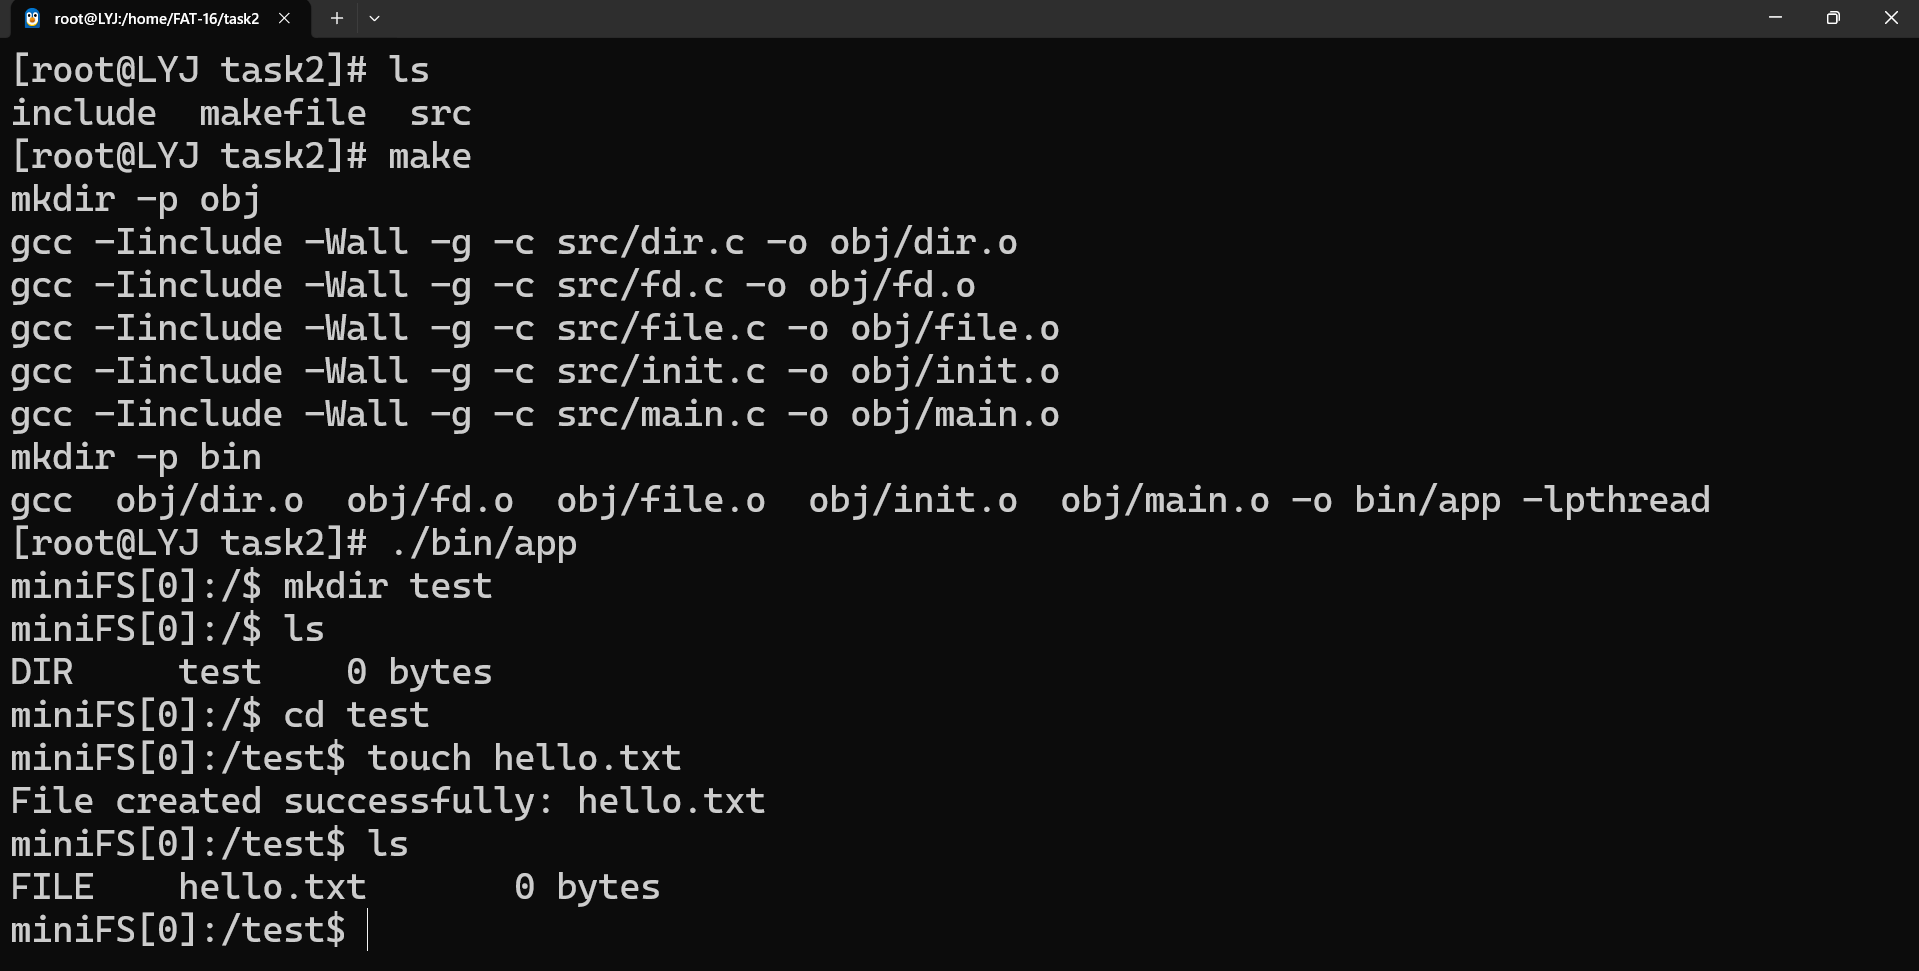
\includegraphics[width=1\textwidth]{figure/task2_common_function.png}
    \caption{文件系统一般操作}
\end{figure}
如上图所示,一般的创建文件夹、创建文件以及切换目录等操作能够正常实现。

\begin{figure}[H]
    \centering
    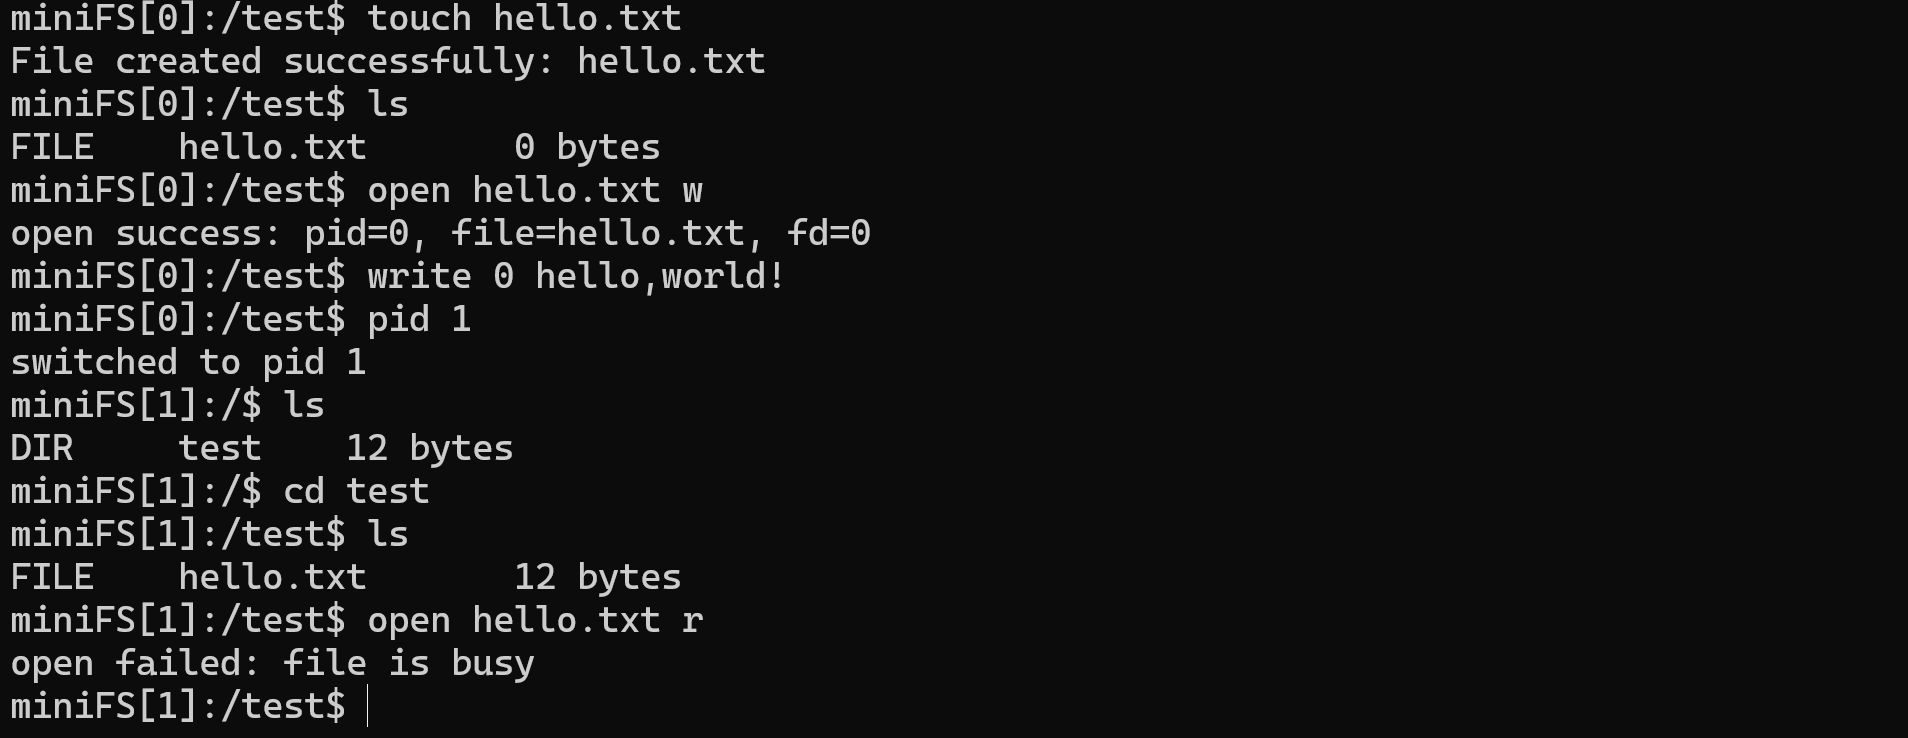
\includegraphics[width = 1\textwidth]{figure/task2_writeonly.png}
    \caption{写进程与读进程互斥}
\end{figure}
如上图所示,当一个写进程(pid=0)打开文件时,切换其他读进程(pid=1)尝试打开文件失败,提示"file is busy",说明能实现写进程互斥访问文件的功能。

\begin{figure}[H]
    \centering
    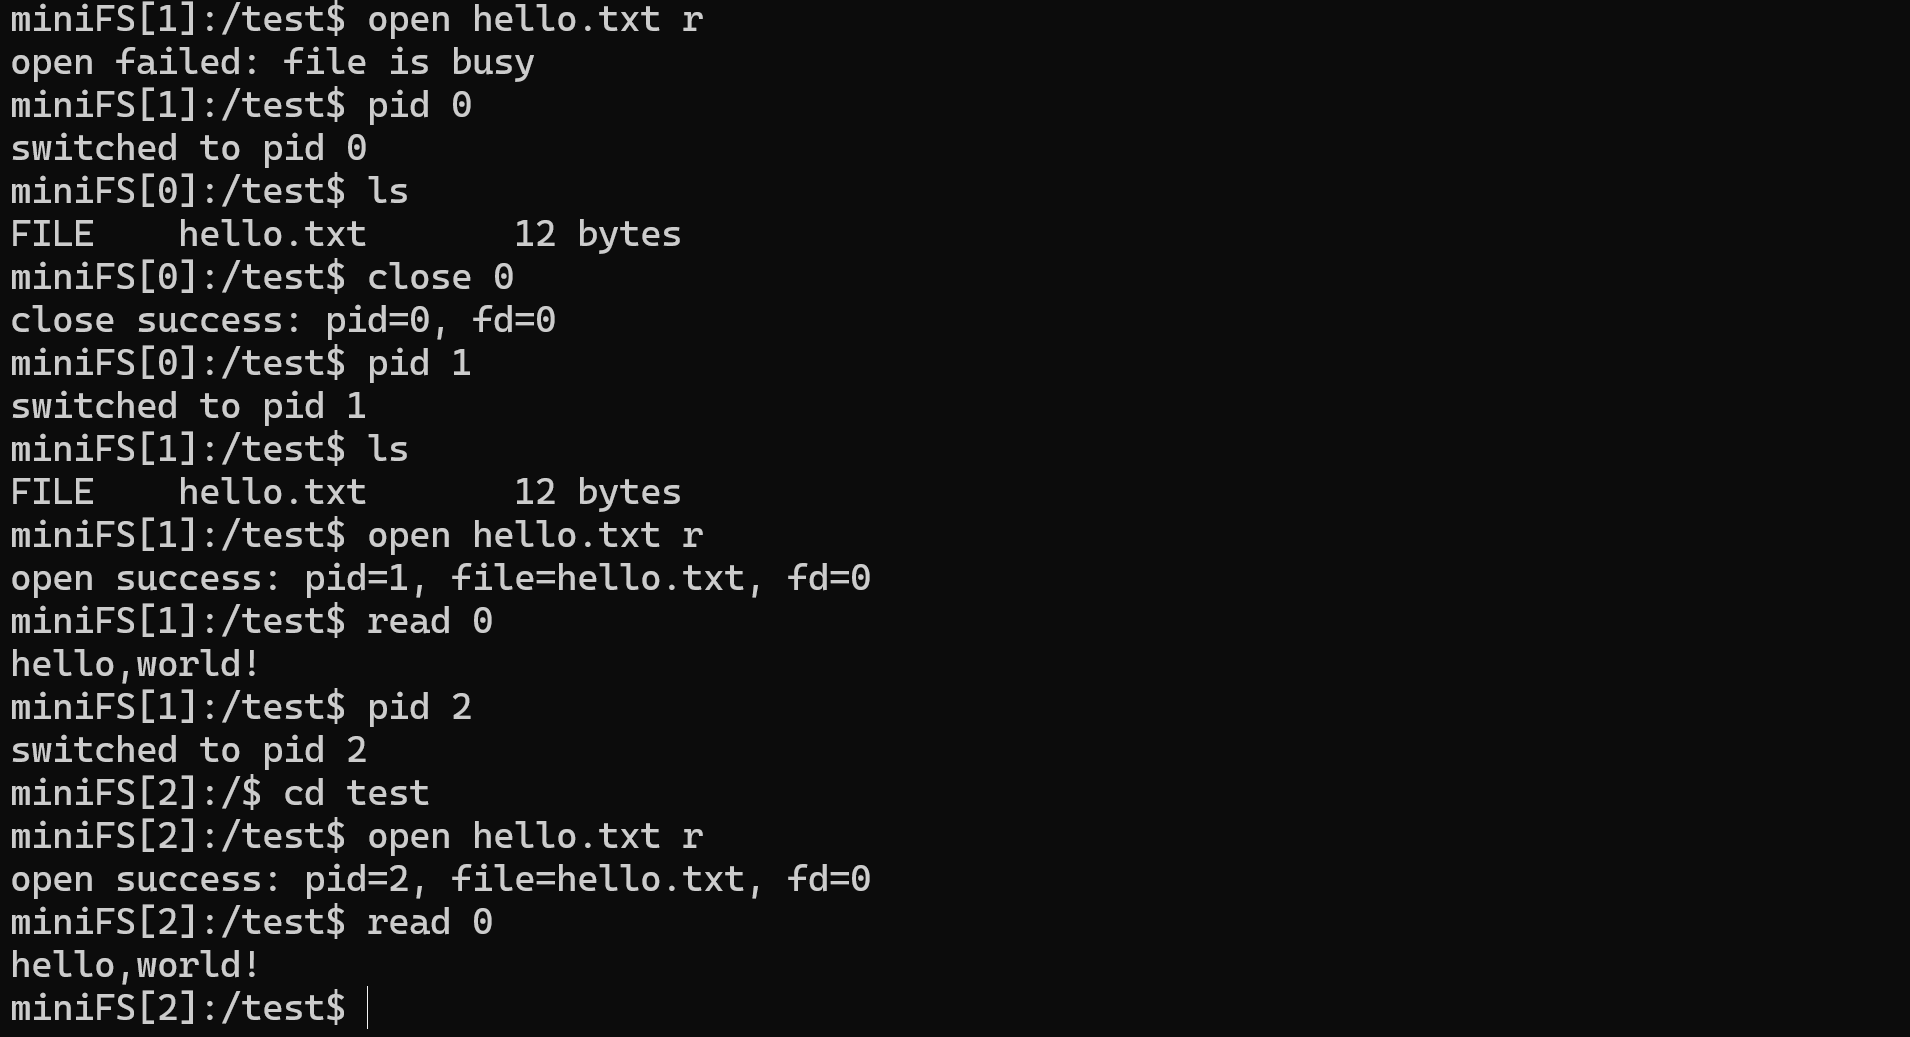
\includegraphics[width = 1\textwidth]{figure/task2_readerShare.png}
    \caption{读进程共享}
\end{figure}
如上图所示,多个读进程(pid=1,2)可以同时访问文件和目录,读取同一个文件的内容。

\begin{figure}[H]
    \centering
    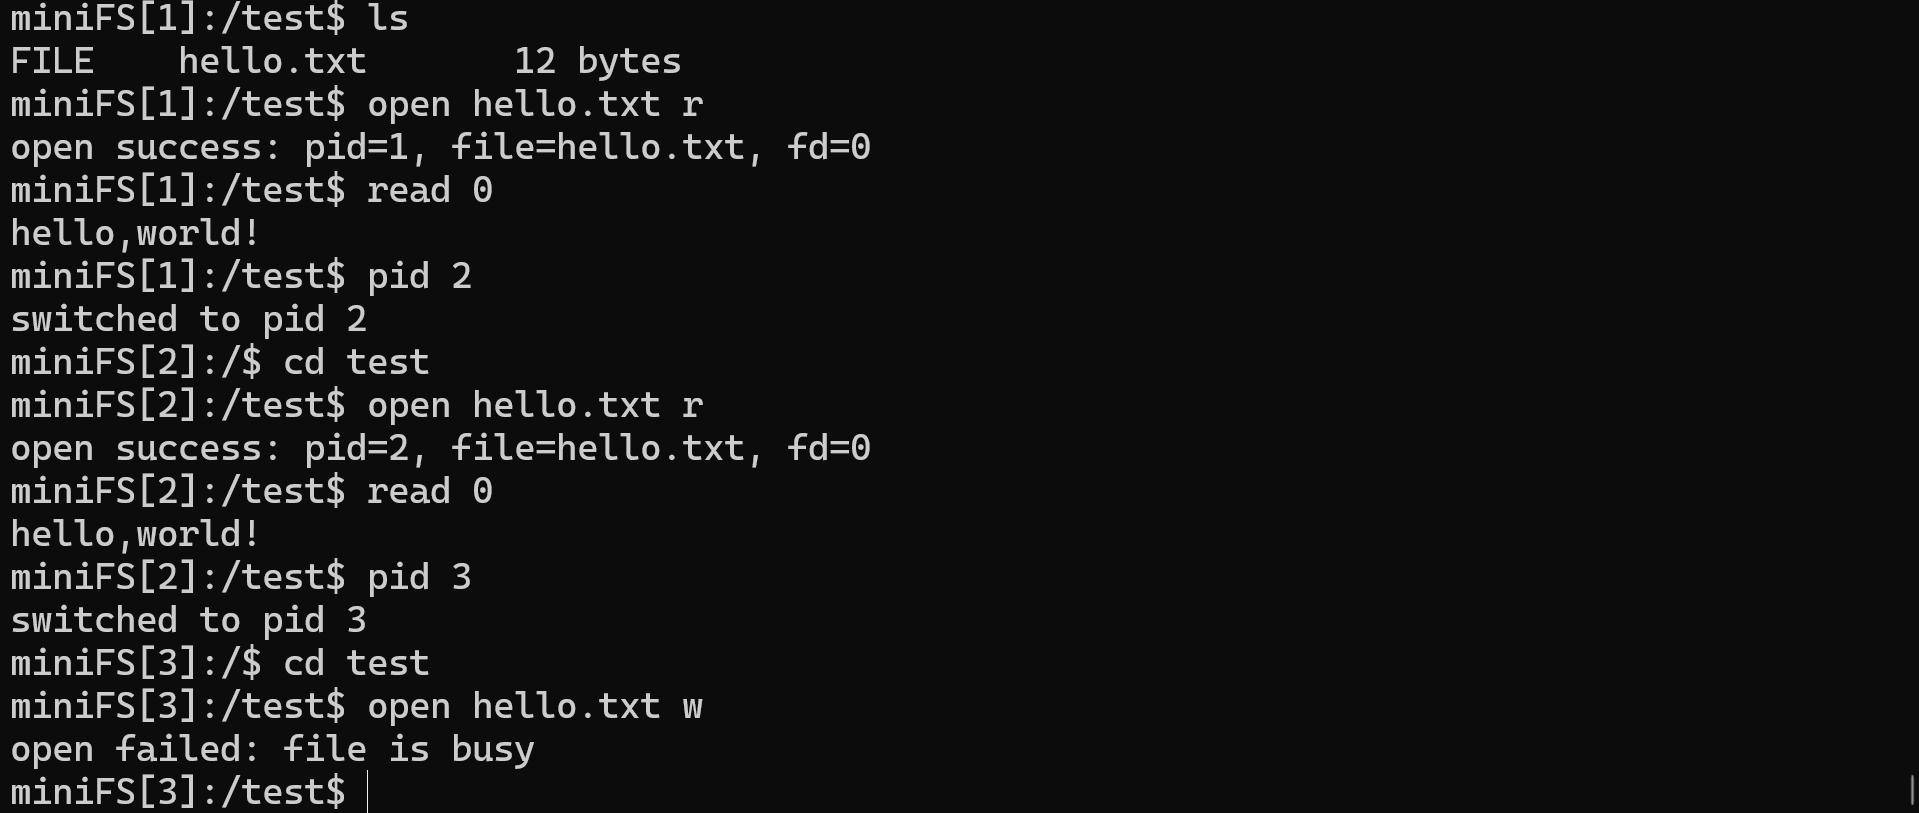
\includegraphics[width = 1\textwidth]{figure/task2_hasreader_writerFail.png}
    \caption{有读进程时写进程访问失败}
\end{figure}
如上图所示,当已经有读进程(pid=1,2)打开文件时,写进程(pid=3)无法访问文件,提示"file is busy",说明能实现读进程与写进程互斥访问文件的功能。
综上所述,该文件系统能够实现多进程之间的读者-写者互斥同步,读写操作均能正确执行,任务二成功完成。